% =====================================================================
% Mechanistic Interpretability Workshop @ ICML 2026
% SHORT PAPER — max 4 pages body, unlimited references + appendix
% DOUBLE-BLIND: no names, affiliations, or identifying info
%
% To compile:
%   pdflatex mechinterp_workshop_2026
%   bibtex   mechinterp_workshop_2026
%   pdflatex mechinterp_workshop_2026
%   pdflatex mechinterp_workshop_2026
% =====================================================================

\documentclass{article}
\usepackage{icml2026}

% ---- Math / symbols ----
\usepackage{amsmath}
\usepackage{amssymb}

% ---- Typography ----
\usepackage{microtype}
\usepackage[T1]{fontenc}

% ---- Figures / tables ----
\usepackage{graphicx}
\usepackage{booktabs}
\usepackage{subcaption}

% ---- Lists ----
\usepackage{enumitem}

% ---- Links ----
\usepackage{xcolor}
\usepackage[colorlinks=true,linkcolor=black,citecolor=blue!60!black,urlcolor=blue!60!black]{hyperref}
\usepackage{url}

% ---- Float control ----
\usepackage{placeins}   % \FloatBarrier

% ---- Inline metric macros ----
\newcommand{\metric}[1]{\textbf{#1}}
% =====================================================================
% TITLE BLOCK
% =====================================================================
\icmltitlerunning{When Does Attention Actually Do Anything?}

\begin{document}

\twocolumn[
  \icmltitle{When Does Attention Actually Do Anything?\\[2pt]
    \large A Large-Scale Diagnostic of Cross-Attention in
    Text-to-Image Diffusion Models}

  \begin{icmlauthorlist}
    \icmlauthor{Anonymous Author(s)}{anon}
  \end{icmlauthorlist}
  \icmlaffiliation{anon}{Anonymous Institution}
  \icmlcorrespondingauthor{Anonymous}{anonymous@example.com}

  \vskip 0.25in
]

% =====================================================================
% ABSTRACT
% =====================================================================
\begin{abstract}
Cross-attention maps in text-to-image diffusion models are routinely
treated as explanations for how text tokens influence image generation.
We test this assumption directly.  Across 16{,}302 controlled
embedding-space interventions on 680 COCO prompts using Stable
Diffusion XL~\citep{podell2023sdxl}, we find that attention maps are
poor spatial predictors of where interventions take effect
(SF-IoU-HR $\approx 0.17$), and that the standard Attention-Delta
Correlation (ADC) metric is partially tautological by construction.
We introduce two decoupled metrics Predictive ADC (P-ADC) and
Latent-Delta Correlation (L-ADC) that remove this circularity.
The strongest finding is structural: \emph{concrete-perceptual}
attributes (color, material) concentrate target-concept attention
roughly three times more than \emph{abstract-stylistic} attributes
(style, atmospheric effect), despite producing comparable image-level
changes (LPIPS).  This asymmetry holds across all intervention
strengths and temporal windows, pointing to a mechanistic difference
in how SDXL's cross-attention processes these two attribute classes.
\end{abstract}

% =====================================================================
% 1. INTRODUCTION
% =====================================================================
\section{Introduction}
\label{sec:intro}

Cross-attention maps in diffusion models nominally show which text
tokens influence each spatial position during denoising.  This
interpretation underpins widely-used methods: Prompt-to-Prompt
editing~\citep{hertz2023prompt}, Attend-and-Excite~\citep{chefer2023attend},
and DAAM~\citep{tang2023daam} all either read model behavior from
attention maps or directly modify them to achieve desired outputs.
More recent work has proposed to use attention as a probe for
implicit reasoning and semantic layout inside generation
pipelines~\citep{kwon2023diffusion,chefer2024hidden}.

But faithfulness is not the same as correlation.  A metric that
compares the attention map computed \emph{during} an intervention
with the change \emph{from} that same intervention is not an
independent test both quantities share the same causal source.
And a map that correlates with output change under ideal conditions
may still fail to localize \emph{where} the change happens spatially.

We construct a clean diagnostic.  We apply training-free CLIP
embedding-arithmetic interventions~\citep{gal2023image} to
SDXL~\citep{podell2023sdxl} and measure five properties of the
resulting attention maps against observed image changes at scale,
across six intervention strengths, four temporal windows, three
prompt categories, and four attribute semantic types.

\textbf{Summary of findings.}
\begin{itemize}[noitemsep,topsep=2pt,leftmargin=1em]
  \item Attention redistribution follows a dose--response curve with
        intervention strength (ACS, $r=-0.218$), saturating near
        $\alpha=1.5$.
  \item The standard ADC metric is partially tautological; our
        decoupled P-ADC is statistically significant
        ($p < 10^{-90}$) but has near-zero effect size
        (mean $\approx 0.10$, std $\approx 0.60$).
  \item Attention maps overlap with changed image regions only
        $\approx$17\% of the time (SF-IoU-HR).
  \item Concrete-perceptual attributes (Color, Material) produce
        attention concentration ${\approx}3\times$ stronger than
        abstract-stylistic attributes (Style, Effect) at matched LPIPS.
\end{itemize}

% =====================================================================
% 2. RELATED WORK
% =====================================================================
\section{Related Work}
\label{sec:related}

\textbf{Attention as explanation.}
\citet{jain2019attention} showed that attention weights are
not reliable explanations in NLP; \citet{wiegreffe2019attention}
partially contested this.  For vision transformers,
\citet{chefer2021transformer} proposed relevancy maps to improve
on raw attention.  In diffusion models, \citet{tang2023daam}
(DAAM) used upsampled cross-attention as spatial explanations and
found modest but non-trivial IoU with segmentation masks---a result
our work replicates and contextualizes at much larger scale.

A crucial distinction, underscored by \citet{ma2024crossself}, is
that \emph{cross-attention} and \emph{self-attention} play
fundamentally different roles in diffusion models: cross-attention
handles semantic \emph{injection} (binding text tokens to spatial
features), while self-attention governs geometric layout and shape
preservation.  \citet{tumanyan2023plug} exploit exactly this
division---they transfer structure via self-attention features while
allowing cross-attention to control appearance.  This division of
labor is a key reason why our SF-IoU-HR metric ($\approx 0.17$)
is low: we are measuring cross-attention against a spatial outcome
that is partly determined by a different attention stream.

\textbf{Editing via attention manipulation.}
\citet{hertz2023prompt} showed that injecting cross-attention maps
from a reference generation enables near-perfect structural
consistency.  \citet{chefer2023attend} directly optimized attention
to improve attribute binding.  \citet{mokady2023null} and
\citet{tumanyan2023plug} used attention features for real-image
inversion and structure transfer.  \citet{brack2023sega} manipulated
concept-token attention for instructable latent editing.
\citet{gandikota2024concept} and \citet{gandikota2024unified}
use concept-level attention routing for controlled concept editing.

\textbf{Semantic latent structure.}
\citet{kwon2023diffusion} found a semantic latent space (h-space)
in diffusion models amenable to arithmetic manipulation.
\citet{orgad2023editing} analyzed how implicit assumptions encoded
in the model can be re-written through attention-layer modifications.
\citet{chefer2024hidden} probed what linguistic concepts the internal
representations of diffusion models encode, finding that early
diffusion layers are highly semantic.

\textbf{Mechanistic interpretability in generative models.}
\citet{elhage2021mathematical} established the mathematical framework
for circuit analysis in transformers, and \citet{conmy2023towards}
proposed automated circuit discovery via activation patching in LLMs.
These techniques are now being ported to diffusion models directly.
\citet{li2026circuit} identify specific cross-attention heads in
diffusion transformers responsible for spatial-relation generation via
causal activation patching.  \citet{chen2026circuits3d} apply the
same framework to 3D diffusion transformers, diagnosing and
stabilizing trajectory failures.  Our work is complementary:
where these studies perform circuit-level causal patching,
we provide a large-scale \emph{observational} diagnostic that
characterizes when and why cross-attention concentration is
meaningful---a necessary precursor to knowing which circuits
to patch.

% =====================================================================
% 3. SETUP
% =====================================================================
\section{Experimental Setup}
\label{sec:setup}

\textbf{Model.}
All experiments use \texttt{stabilityai/stable-diffusion-xl-base-1.0}
(SDXL)~\citep{podell2023sdxl}, 50 DDIM~\citep{song2021ddim} steps,
guidance scale 7.5, seed 42, \texttt{float16}.  Cross-attention
probabilities are extracted via hooks at every denoising step
(verified: $\sum_j p_{ij} = 1.0$, MAE $< 10^{-6}$).

\textbf{Interventions.}
For each prompt we identify a \emph{target concept} (a noun) and
an \emph{injection attribute}.  The attribute is injected via CLIP
embedding arithmetic:
\[
  \delta \;=\; \mathrm{Enc}(\text{attr}) - \mathrm{Enc}(\text{concept}),
\]
scaled by strength $\alpha \in \{0.25, 0.50, 0.75, 1.0, 1.5, 2.0\}$
and applied only within a temporal window of denoising steps
(four windows: 50--35, 35--20, 20--5, 45--5).
No fine-tuning is performed.

\textbf{Dataset.}
We sample 680 COCO 2017 captions~\citep{lin2014coco} spanning three
categories \textit{Simple} (50 prompts), \textit{Compositional}
(451), and \textit{Conflicting} (158).  Twenty attributes are grouped
into four semantic clusters: \textit{Color} (blue, red, golden,
silver, neon green), \textit{Material} (glass, stone, wooden,
metallic, velvet), \textit{Style} (baroque, cyberpunk, futuristic,
minimalist, ancient), \textit{Effect} (fiery, frozen, glowing, misty,
shadowy).  Every prompt $\times$ attribute pair receives all 24
conditions (6 strengths $\times$ 4 windows), yielding \textbf{16,302
total interventions}.

\textbf{Metrics.}
\begin{itemize}[noitemsep,topsep=2pt,leftmargin=*]

\item \metric{ACS} (Attention Concentration Score): relative change
  in target-token attention mass,
  $\mathrm{ACS} = (\bar{a}^{\mathrm{interv}} - \bar{a}^{\mathrm{base}}) / \bar{a}^{\mathrm{base}}$.
  Negative $\implies$ attention \emph{disperses} from the target.

\item \metric{ADC} (Attention-Delta Correlation): Pearson $r$ between
  per-step intervention attention and per-step attention-delta.
  Retained for comparison; note both quantities derive from the same
  forward pass, introducing circularity.

\item \metric{P-ADC} (\emph{ours}): Pearson $r$ between
  \emph{baseline-pass} attention (pre-intervention) and the per-step
  change induced by the intervention. Predictor and outcome are
  from separate forward passes.

\item \metric{L-ADC} (\emph{ours}): Pearson $r$ between baseline
  attention and per-step latent L2-divergence between baseline and
  intervention trajectories.

\item \metric{SF-IoU-HR} (DAAM-style~\citep{tang2023daam}): IoU
  between the attention heatmap upsampled to image resolution and
  the pixel-change mask. Also computed at native resolution
  (SF-IoU).

\end{itemize}
% =====================================================================
% 4. RESULTS
% =====================================================================
\section{Results}
\label{sec:results}

\subsection{Dose-Response and the Limits of ACS}

Table~\ref{tab:by_strength} summarizes metrics across intervention
strengths.  ACS scales monotonically with $\alpha$ ($r=-0.218$,
$p < 10^{-3}$, Cohen's $d=1.12$ for $\alpha\!=\!0.25$
vs.\ $\alpha\!=\!2.0$), then saturates above $\alpha=1.5$.
LPIPS increases monotonically.

\textbf{What does not scale is predictive power.}
P-ADC stays near zero (mean $\approx 0.097$, std $\approx 0.60$)
across all strengths.  It is statistically nonzero ($t=18.9$,
$p < 10^{-90}$, $N=15{,}798$) but the large standard deviation
makes it an unreliable per-sample predictor.  SF-IoU-HR
plateaus at 0.165--0.180: attention heatmaps overlap with changed
pixels only $\approx$17\% of the time.

\begin{table}[t]
\centering
\caption{Metrics by intervention strength $\alpha$.
         Means over all prompts, attributes, and windows.}
\label{tab:by_strength}
\vskip 0.05in
\setlength{\tabcolsep}{3.5pt}
\footnotesize
\begin{tabular}{@{}lcccccc@{}}
\toprule
$\alpha$ & ACS & P-ADC & L-ADC & SF-IoU-HR & LPIPS & $N$ \\
\midrule
0.25 & $-0.105$ & $0.100$ & $-0.099$ & $0.165$ & $0.067$ & 2636 \\
0.50 & $-0.174$ & $0.098$ & $-0.084$ & $0.166$ & $0.096$ & 2634 \\
0.75 & $-0.217$ & $0.097$ & $-0.072$ & $0.168$ & $0.120$ & 2632 \\
1.00 & $-0.243$ & $0.098$ & $-0.063$ & $0.170$ & $0.142$ & 2632 \\
1.50 & $-0.259$ & $0.099$ & $-0.047$ & $0.176$ & $0.182$ & 2632 \\
2.00 & $-0.248$ & $0.096$ & $-0.035$ & $0.180$ & $0.220$ & 2632 \\
\bottomrule
\end{tabular}
\end{table}

\subsection{Attribute Type Predicts Attention Engagement}

The clearest signal is not strength- or timing-dependent.
As shown in Table~\ref{tab:by_cluster} and Figure~\ref{fig:clusters},
\emph{attribute semantic type} is the dominant predictor of ACS.
Color and Material attributes consistently show strong attention
concentration (ACS $\approx -0.31$ and $-0.35$, respectively).
Style and Effect attributes produce roughly \textbf{three times
weaker} attention shifts (ACS $\approx -0.11$ and $-0.10$), despite
similar LPIPS values ($0.130$--$0.150$ vs.\ $0.131$--$0.138$).

\begin{table}[t]
\centering
\caption{Metrics by attribute cluster.  Color and Material
         concentrate target attention ${\sim}3\times$ more than
         Style and Effect, at matched LPIPS.}
\label{tab:by_cluster}
\vskip 0.05in
\setlength{\tabcolsep}{3.5pt}
\footnotesize
\begin{tabular}{@{}lcccc@{}}
\toprule
Cluster & ACS & P-ADC & SF-IoU-HR & LPIPS \\
\midrule
Color    & $-0.306 \pm 0.13$ & $0.090 \pm 0.60$ & $0.177$ & $0.150$ \\
Material & $-0.349 \pm 0.16$ & $0.096 \pm 0.59$ & $0.167$ & $0.132$ \\
Style    & $-0.106 \pm 0.18$ & $0.088 \pm 0.58$ & $0.179$ & $0.138$ \\
Effect   & $-0.098 \pm 0.19$ & $0.118 \pm 0.62$ & $0.163$ & $0.131$ \\
\bottomrule
\end{tabular}
\end{table}

This asymmetry replicates across all prompt categories, strength
levels, and temporal windows.  It is not driven by differences in
LPIPS: the image-level perturbation is comparable, but only
concrete-perceptual attributes trigger proportional attention
concentration.  One account: concrete token concepts (``blue'',
``wooden'') correspond to tighter, more localized CLIP embeddings,
so the steering direction $\delta$ lands in a region of embedding
space that maps to focused cross-attention redistribution.  Abstract
concepts (``baroque'', ``misty'') have diffuse embeddings; the
resulting $\delta$ changes the latent trajectory without producing
a correspondingly localized attention shift.  This is consistent
with \citet{wang2025attnoverlap}, who show that excessive
cross-attention \emph{spread and overlap} directly causes attribute
binding failures and entity-missing artefacts---our Style and Effect
attributes, with their near-zero ACS, sit precisely in this
failure-prone regime.  We leave direct testing of this account
via text-encoder probing or targeted attention knockout as future work.

\subsection{Temporal Window Effect}

Table~\ref{tab:by_window} shows metrics by intervention window.
ACS is stable (range 0.199--0.223) across all four windows,
suggesting that \emph{when} the intervention is applied has little
effect on how much attention concentrates.  SF-IoU-HR shows a small
but consistent gradient: 0.156 in the early window (steps 50--35,
structural phase) rising to 0.177 in the late and full windows.
LPIPS varies strongly: early interventions reshape global structure
(LPIPS $=0.242$) while late interventions affect fine detail only
(LPIPS $=0.042$).

\begin{table}[t]
\centering
\caption{Metrics by temporal intervention window.
         DDIM step ranges out of 50 total steps.}
\label{tab:by_window}
\vskip 0.05in
\setlength{\tabcolsep}{3.5pt}
\footnotesize
\begin{tabular}{@{}lcccc@{}}
\toprule
Window & ACS & P-ADC & SF-IoU-HR & LPIPS \\
\midrule
Early (50--35) & $-0.223$ & $-0.065$ & $0.156$ & $0.242$ \\
Mid   (35--20) & $-0.203$ & $+0.275$ & $0.170$ & $0.083$ \\
Late  (20--5)  & $-0.199$ & $-0.076$ & $0.177$ & $0.042$ \\
Full  (45--5)  & $-0.206$ & $+0.258$ & $0.177$ & $0.183$ \\
\bottomrule
\end{tabular}
\end{table}

% Flush all floats before the spanning figure
% \FloatBarrier

\begin{figure*}[t]
\centering
\begin{subfigure}[b]{0.47\linewidth}
  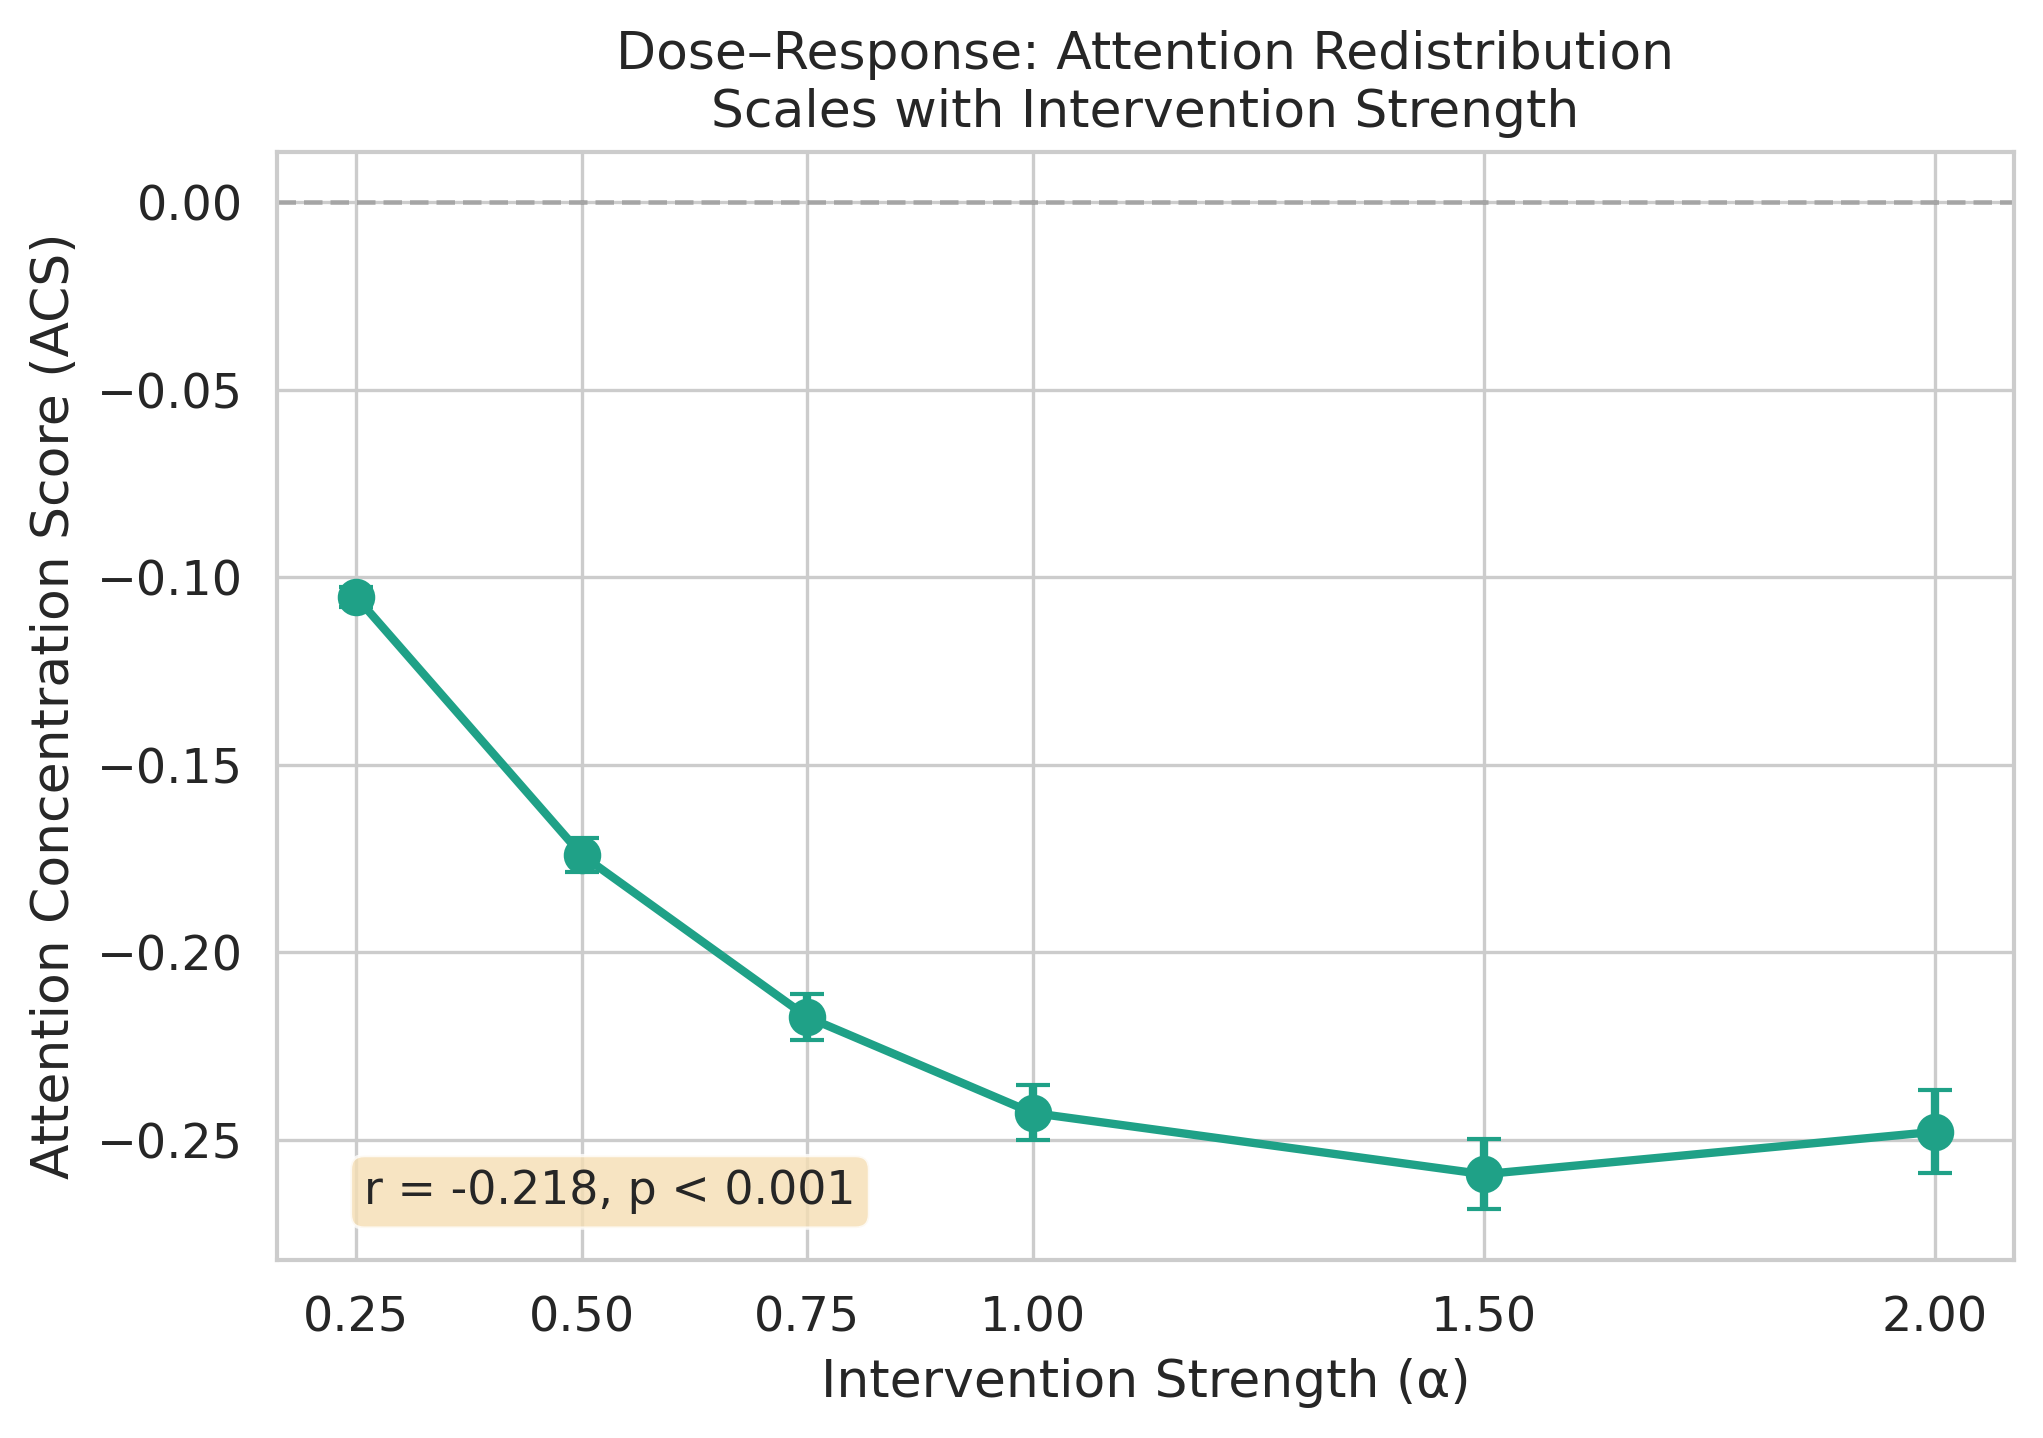
\includegraphics[width=\linewidth]{paper_figures_v2/fig1_acs_vs_strength.png}
  \caption{ACS vs.\ $\alpha$.  Error bars = 95\% CI.
           Monotonic; saturates at $\alpha\!\approx\!1.5$
           ($r=-0.218$, Cohen's $d=1.12$).}
  \label{fig:acs_strength}
\end{subfigure}
\hfill
\begin{subfigure}[b]{0.47\linewidth}
  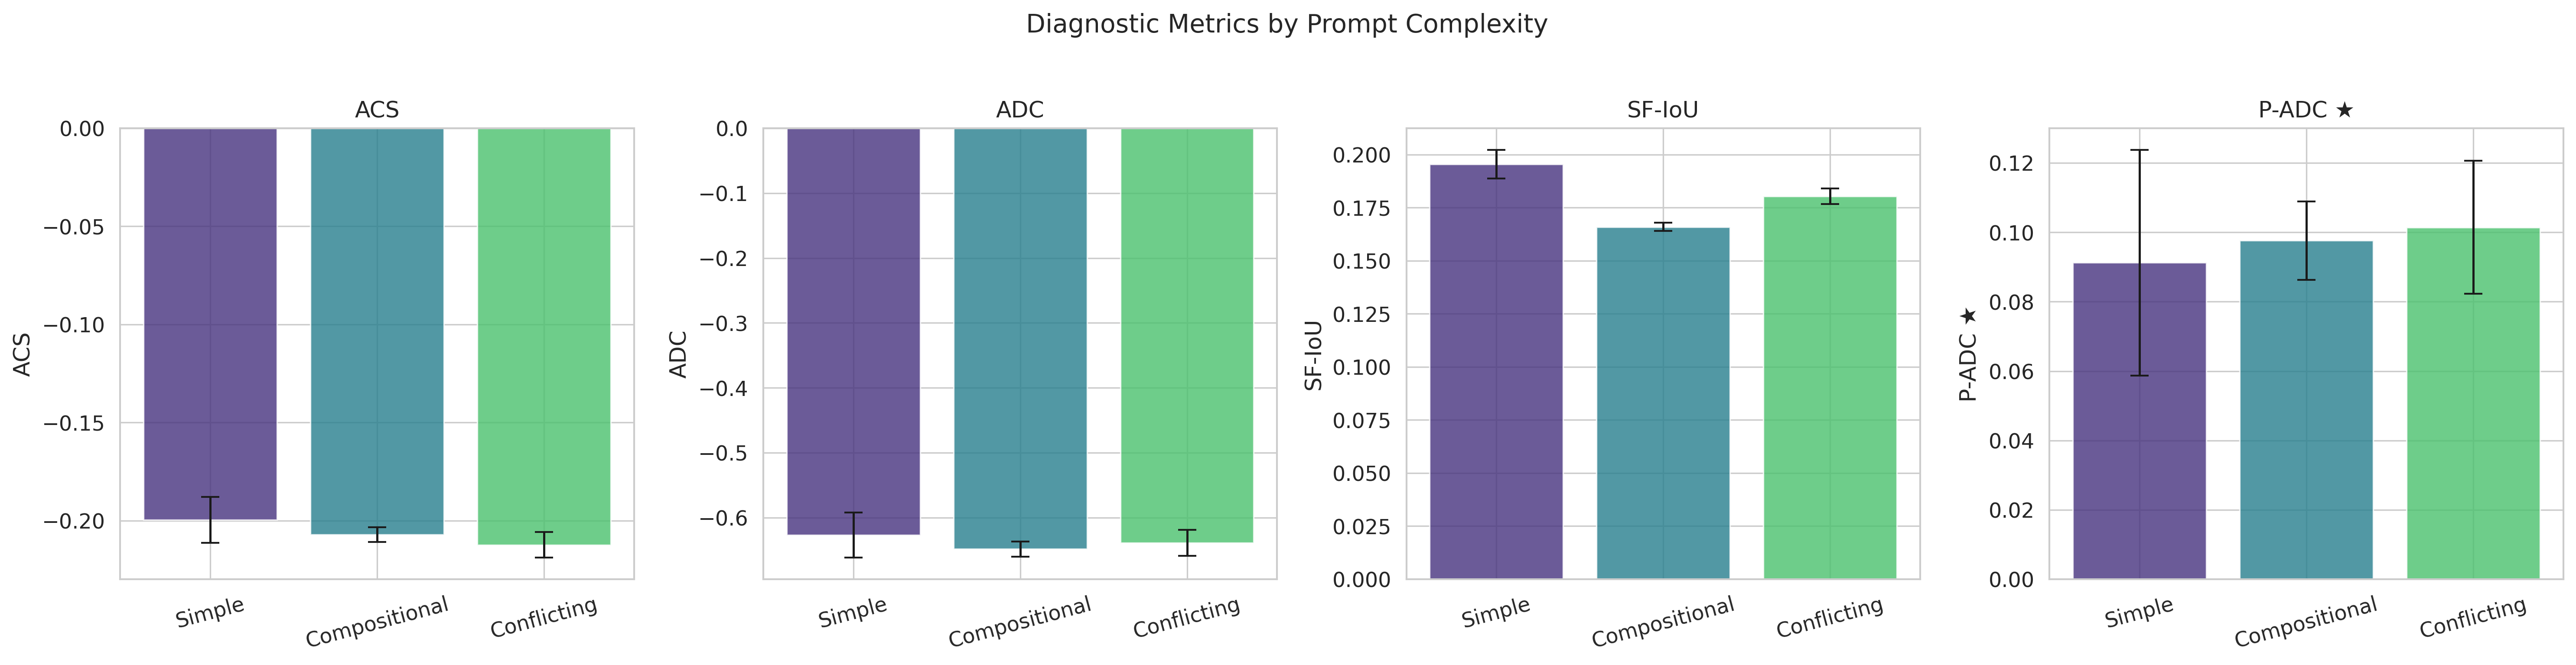
\includegraphics[width=\linewidth]{paper_figures_v2/fig8_category_comparison.png}
  \caption{ACS by attribute cluster and prompt category.
           Color/Material gap (${\sim}3\times$) dominates
           any category-level effect.}
  \label{fig:clusters}
\end{subfigure}
\caption{\textbf{Key findings.}
  \textbf{(a)}~Attention redistribution scales with strength and
  saturates a dose--response curve.
  \textbf{(b)}~Attribute semantic type, not prompt category,
  is the primary predictor of attention engagement.}
\label{fig:main}
\end{figure*}

% =====================================================================
% 5. DISCUSSION
% =====================================================================
\section{Discussion}
\label{sec:discussion}

\textbf{The ADC metric has a structural problem.}
ADC values near $-1.0$ for Color and Material clusters arise because
the metric correlates attention \emph{from} the intervention pass
with attention deltas \emph{from} the same pass.  P-ADC breaks this
by using baseline-pass attention as the predictor.  The resulting
near-zero P-ADC (mean $\approx 0.10$) is itself a result: knowing
where the model naturally attends to a concept tells us little about
where an intervention will concentrate its effect per-sample.

\textbf{Attention maps are spatially imprecise.}
SF-IoU-HR $\approx 0.17$ means roughly 83\% of high-attention pixels
do not coincide with the pixels that actually changed.  This is
consistent with DAAM's findings on SD~1.4~\citep{tang2023daam} and
with \citet{chefer2024hidden}'s observation that internal diffusion
representations are only loosely spatially grounded.  A structural
explanation follows from \citet{ma2024crossself}: cross-attention
injects \emph{semantic} signal into the residual stream, but the
actual spatial realization of that signal is mediated downstream
by self-attention layers.  Measuring cross-attention against a
pixel-change mask conflates two separate computations.  Interventions
\emph{work}---LPIPS increases monotonically---but the cross-attention
map is a poor spatial readout of where the effect lands precisely
because spatial structure is handled elsewhere.

\textbf{The attribute-type asymmetry is the most actionable finding.}
Color and Material: $|\text{ACS}| \approx 0.33$.  Style and Effect:
$|\text{ACS}| \approx 0.10$.  LPIPS $\approx 0.13$--$0.15$ for both
groups.  This matches the prediction of~\citet{kwon2023diffusion}
that concrete visual concepts occupy more compact latent
neighborhoods.  A direct mechanism test via targeted attention
knockout for Color vs.\ Style tokens, or CLIP embedding-space
geometry analysis, is a natural next step.  The causal patching
methodology for such experiments in diffusion models has been
demonstrated by \citet{li2026circuit} and \citet{chen2026circuits3d},
providing a ready-made experimental framework.

\textbf{Limitations.}
(1)~Single model (SDXL base 1.0); cross-model generalization to
SD~3~\citep{esser2024scaling} or FLUX is untested.
(2)~P-ADC establishes predictive correlation, not causality.
(3)~COCO prompts may not represent real-world generation requests.

% =====================================================================
% 6. CONCLUSION
% =====================================================================
\section{Conclusion}
\label{sec:conclusion}

We ran 16{,}302 controlled interventions on SDXL and measured
whether cross-attention maps faithfully predict intervention effects.
They do not, spatially (SF-IoU-HR $\approx 0.17$), and the standard
ADC metric overstates their predictive power via circularity.
The most replicable finding is structural: Color and Material
attributes concentrate target-concept attention three times more
strongly than Style and Effect attributes, at matched image-level
perturbation.  This asymmetry is a concrete, testable hypothesis
about how SDXL's cross-attention differentially processes concrete
vs.\ abstract token meanings, and motivates targeted causal
ablation experiments.  Code and data:
\url{https://anonymous.4open.science/r/diffusion-detective}.

% =====================================================================
% REFERENCES — \clearpage first to flush ALL pending floats
% =====================================================================
% \clearpage
\bibliographystyle{abbrvnat}
\bibliography{mechinterp_workshop_2026_refs}

% =====================================================================
% APPENDIX (unlimited; reviewers not required to read)
% =====================================================================
\clearpage
\appendix
\onecolumn

\section{Full Metric Tables}
\label{app:tables}

\begin{table}[h]
\centering
\caption{All metrics by intervention strength (mean; std in parentheses).}
\small
\begin{tabular}{@{}lccccccc@{}}
\toprule
$\alpha$ & ACS & ADC & P-ADC & L-ADC & SF-IoU & SF-IoU-HR & LPIPS \\
\midrule
0.25 & $-0.105$ & $-0.610$ & $0.100$ & $-0.099$ & $0.162$ & $0.165$ & $0.067$ \\
     & $(0.070)$ & $(0.517)$ & $(0.594)$ & $(0.793)$ & $(0.110)$ & $(0.096)$ & $(0.072)$ \\[2pt]
0.50 & $-0.174$ & $-0.690$ & $0.098$ & $-0.084$ & $0.165$ & $0.166$ & $0.096$ \\
     & $(0.121)$ & $(0.528)$ & $(0.596)$ & $(0.799)$ & $(0.110)$ & $(0.098)$ & $(0.089)$ \\[2pt]
0.75 & $-0.217$ & $-0.695$ & $0.097$ & $-0.072$ & $0.169$ & $0.168$ & $0.120$ \\
     & $(0.160)$ & $(0.566)$ & $(0.597)$ & $(0.801)$ & $(0.110)$ & $(0.099)$ & $(0.102)$ \\[2pt]
1.00 & $-0.243$ & $-0.677$ & $0.098$ & $-0.063$ & $0.172$ & $0.170$ & $0.142$ \\
     & $(0.192)$ & $(0.611)$ & $(0.599)$ & $(0.802)$ & $(0.109)$ & $(0.098)$ & $(0.114)$ \\[2pt]
1.50 & $-0.259$ & $-0.625$ & $0.099$ & $-0.047$ & $0.179$ & $0.176$ & $0.182$ \\
     & $(0.245)$ & $(0.685)$ & $(0.598)$ & $(0.801)$ & $(0.107)$ & $(0.097)$ & $(0.130)$ \\[2pt]
2.00 & $-0.248$ & $-0.569$ & $0.096$ & $-0.035$ & $0.183$ & $0.180$ & $0.220$ \\
     & $(0.291)$ & $(0.741)$ & $(0.600)$ & $(0.801)$ & $(0.104)$ & $(0.095)$ & $(0.141)$ \\
\bottomrule
\end{tabular}
\end{table}

\begin{table}[h]
\centering
\caption{All metrics by prompt category.}
\small
\begin{tabular}{@{}lcccccc@{}}
\toprule
Category & ACS & P-ADC & L-ADC & SF-IoU-HR & LPIPS & $N_\text{prompts}$ \\
\midrule
Compositional & $-0.207$ & $0.098$ & $-0.046$ & $0.165$ & $0.137$ & 451 \\
Conflicting   & $-0.212$ & $0.102$ & $-0.022$ & $0.178$ & $0.138$ & 158 \\
Simple        & $-0.200$ & $0.091$ & $-0.394$ & $0.187$ & $0.141$ & 50  \\
\bottomrule
\end{tabular}
\end{table}

\begin{table}[h]
\centering
\caption{Full metrics by temporal window.}
\small
\begin{tabular}{@{}lcccccc@{}}
\toprule
Window & ACS & ADC & P-ADC & L-ADC & SF-IoU-HR & LPIPS \\
\midrule
Early (50--35) & $-0.223$ & $-0.701$ & $-0.065$ & $+0.033$ & $0.156$ & $0.242$ \\
Mid   (35--20) & $-0.203$ & $-0.626$ & $+0.275$ & $-0.093$ & $0.170$ & $0.083$ \\
Late  (20--5)  & $-0.199$ & $-0.674$ & $-0.076$ & $-0.202$ & $0.177$ & $0.042$ \\
Full  (45--5)  & $-0.206$ & $-0.577$ & $+0.258$ & $-0.005$ & $0.177$ & $0.183$ \\
\bottomrule
\end{tabular}
\end{table}

\section{Statistical Tests}
\label{app:stats}

\begin{itemize}[leftmargin=1.5em]
  \item ACS $\neq 0$: significant at all strengths ($p < 10^{-100}$).
  \item P-ADC $\neq 0$: $t=18.9$,\; $p < 10^{-90}$,\; $N=15{,}798$.
        Mean $= 0.098$, std $= 0.60$; effect size is small.
  \item $r(\text{ACS},\,\alpha) = -0.218$,\; $p < 10^{-3}$
        (dose--response).
  \item $r(|\text{ACS}|,\,\text{LPIPS}) = +0.63$,\; $p < 10^{-100}$.
  \item Cohen's $d$ (ACS: $\alpha\!=\!0.25$ vs.\ $\alpha\!=\!2.0$)
        $= 1.12$.
  \item ADC $\neq 0$: $p < 10^{-100}$; partially tautological
        (see Section~\ref{sec:setup}).
\end{itemize}

\section{Implementation Details}
\label{app:impl}

\noindent\textbf{Hardware.}
Single NVIDIA V100 (16\,GB). Throughput $\approx 45$ interventions
per GPU-hour.

\noindent\textbf{SDXL settings.}
\texttt{stabilityai/stable-diffusion-xl-base-1.0}, 50 DDIM steps,
guidance scale 7.5, seed 42, \texttt{float16}.

\noindent\textbf{Attention extraction.}
Hooks on all \texttt{CrossAttention} modules; probability rows
verified to sum to 1.0 within MAE $< 10^{-6}$.

\noindent\textbf{CLIP metric.}
\texttt{openai/clip-vit-base-patch32}~\citep{radford2021clip}.
$\Delta$-CLIP uses the directional formulation from
StyleGAN-NADA~\citep{gal2023stylegan}.

\noindent\textbf{LPIPS.}
VGG backbone, \texttt{torchmetrics}
implementation~\citep{zhang2018lpips}.

\noindent\textbf{SF-IoU-HR.}
Attention maps mean-pooled across heads and steps, bilinearly
upsampled to $1024\!\times\!1024$ (DAAM
protocol~\citep{tang2023daam}), binarized at 75th percentile.
Same percentile threshold applied to the pixel-change mask.

\end{document}
